\documentclass{article}
\usepackage[submission]{colm2026_conference}

\usepackage{microtype}
\usepackage{hyperref}
\usepackage{url}
\usepackage{booktabs}
\usepackage{amsmath}
\usepackage{amssymb}
\usepackage{graphicx}
\usepackage{multirow}
\usepackage{xcolor}
\usepackage{subcaption}
\usepackage{enumitem}
\usepackage{amsthm}
\newtheorem{theorem}{Theorem}

\usepackage{lineno}

\definecolor{darkblue}{rgb}{0, 0, 0.5}
\hypersetup{colorlinks=true, citecolor=darkblue, linkcolor=darkblue, urlcolor=darkblue}

\newcommand{\fix}{\marginpar{FIX}}
\newcommand{\new}{\marginpar{NEW}}

\title{How Reliable Are VLM Judges? Conformal Prediction Reveals Task-Dependent Uncertainty in Multimodal Evaluation}

\author{Anonymous authors\\Paper under double-blind review}

\begin{document}

\ifcolmsubmission
\linenumbers
\fi

\maketitle

\begin{abstract}
Vision-language models (VLMs) are increasingly used as automated judges for multimodal systems, yet their scores provide no indication of reliability. We study this problem through conformal prediction, a distribution-free framework that converts a judge's point score into a calibrated prediction interval using only score-token log-probabilities, with no retraining. 
We present the first systematic analysis of conformal prediction for VLM-as-a-Judge across 3 judges and 14 visual task categories. Our results show that evaluation uncertainty is strongly task-dependent: intervals cover $\sim 40\%$ of the score range for aesthetics and natural images but expand to $\sim 70\%$ for chart and mathematical reasoning, yielding a quantitative reliability map for multimodal evaluation. 
We further identify a previously unrecognized failure mode, \emph{ranking-scoring decoupling}, where judges achieve high ranking correlation while producing wide, uninformative intervals, correctly ordering responses but failing to assign reliable absolute scores. 
Finally, we show that interval width is driven primarily by task difficulty and annotation quality, i.e., the same judge and method yield $4.5\times$ narrower intervals on a clean, multi-annotator captioning benchmark. 
\end{abstract}

\section{Introduction}
\label{sec:intro}

Vision-Language Models (VLMs) are increasingly used as automated judges to evaluate multimodal AI systems~\citep{chen2024mllmasajudge,li2024vlrewardbench}. This \emph{VLM-as-a-Judge} paradigm extends LLM-based evaluation to tasks requiring visual understanding, including chart comprehension, visual question answering, image captioning, and AI-generated image quality. As multimodal agents are deployed in high-stakes settings such as medical imaging, web navigation, and document analysis, the reliability of these evaluations becomes critical. 

However, VLM judges produce only point scores, offering no indication of reliability. A score of four out of five (4/5) may reflect confident correctness or substantial uncertainty, yet users cannot distinguish between the two. This limitation is exacerbated in multimodal settings, where errors can arise from both visual perception and language reasoning. For example, evaluating a chart-based answer requires visual parsing, data extraction, and reasoning, each introducing compounding uncertainty. Empirically, this reliability gap is significant. On the MLLM-as-a-Judge benchmark~\citep{chen2024mllmasajudge}, state-of-the-art VLM judges achieve only 32--34\% exact agreement with human ratings on a 5-point scale, and 24--30\% of predictions deviate by 2 or more points. Correlation metrics remain modest ($\rho = 0.30$--$0.46$), providing limited assurance about per-instance reliability. Existing evaluation metrics thus fail to indicate when a judge's score can be trusted.

We address this problem using conformal prediction~\citep{vovk2005algorithmic}, a post-hoc, distribution-free framework that converts point scores into calibrated prediction intervals with provable coverage guarantees. Given a target coverage (e.g., 90\%), these intervals contain the true human score with high probability, without requiring model retraining or assumptions on error distributions. Conformal prediction operates directly on score-token log-probabilities, making it readily applicable to existing VLM judge pipelines. While prior work~\citep{sheng2025analyzing} demonstrates the effectiveness of conformal prediction for text-only LLM judges, extending it to multimodal evaluation introduces new challenges: (i) cross-modal uncertainty from visual and textual reasoning, (ii) discrete single-annotator ground truth, (iii) substantial task heterogeneity across visual domains, and (iv) varying levels of log-probability access across models. Standard metrics such as correlation and accuracy fail to capture evaluation reliability. 

We present a systematic study of conformal prediction for VLM-based evaluation. Our contribution is not the application of conformal prediction itself, but the identification of task-dependent uncertainty structure and a fundamental decoupling between ranking quality and scoring reliability in multimodal evaluation. We show that high correlation does not imply reliable absolute scores, and that uncertainty is primarily driven by task ambiguity and annotation quality rather than model scale. Our key findings are:

\begin{itemize}[leftmargin=*,itemsep=0pt,topsep=0pt]

\item \textbf{Task-dependent uncertainty:} Prediction interval width varies by up to 70\% across tasks. Vision-heavy tasks such as charts and mathematical reasoning yield substantially wider intervals than natural image or aesthetics tasks, providing a quantitative reliability map.

\item \textbf{Ranking-scoring decoupling:} We identify a previously unrecognized failure mode where judges achieve strong ranking correlation while producing wide, uninformative intervals. That is, they correctly order responses but fail to assign reliable absolute scores.

\item \textbf{Role of data quality:} Interval width is primarily driven by task difficulty and annotation quality rather than the conformal method. The same judge and method produce $4.5\times$ narrower intervals on a clean, multi-annotator captioning benchmark.

\item \textbf{Task-conditional calibration:} We show that conditioning on task difficulty (Mondrian CP) yields narrower intervals for easy tasks while improving coverage for hard tasks. \vspace{-3pt}

\end{itemize}

\section{Related work}
\label{sec:related}

\textbf{LLM-as-a-Judge.}
Using LLMs as automated evaluators has become a standard approach for assessing natural language generation~\citep{zheng2023judging,liu2023geval}. G-Eval~\citep{liu2023geval} uses chain-of-thought prompting with GPT-4 to score text quality and improves correlation with human judgments over metrics such as ROUGE and BERTScore. MT-Bench and Chatbot Arena~\citep{zheng2023judging} establish pairwise evaluation and reveal systematic biases including position and verbosity bias. SocREval~\citep{he2024soceval} focuses on reasoning. 

\textbf{VLM-as-a-Judge.}
This paradigm has been extended to multimodal evaluation. \citet{chen2024mllmasajudge} introduce the MLLM-as-a-Judge benchmark with 14 visual task categories and report limited alignment with human judgments. LLaVA-Critic~\citep{xiong2024llavacritic} trains a dedicated multimodal judge, while VL-RewardBench~\citep{li2024vlrewardbench} shows that a large fraction of errors are perceptual rather than reasoning-driven. 

\textbf{Uncertainty in LLM-based evaluation.}
Recent work studies confidence and uncertainty in LLM judgments. \citet{wagner2024llmconfidence} derive confidence scores from token probabilities and show weak correlation with accuracy. \citet{xie2025boosted} use token probabilities for calibration and propose boosted conformal methods. Other approaches rely on self-reported confidence~\citep{xiong2024selfconsistency} or consistency across multiple generations~\citep{tian2023consistency}, both with known limitations. \citet{sheng2025analyzing} apply conformal prediction to text-only LLM judges and show that calibrated intervals improve reliability. 

\textbf{Conformal prediction.}
Conformal prediction provides distribution-free uncertainty estimates with coverage guarantees~\citep{vovk2005algorithmic}. Prior work applies it mainly to classification tasks such as multiple-choice QA and response selection~\citep{kumar2023conformal,zhang2024conformal,su2024api,vishwakarma2025conformal,quach2024conformal,mohri2024language,wang2024cpsele,kladny2025conformal}. \citet{jung2024conformal} study preference alignment through conformalized risk control. 

\section{Uncertainty Quantification for VLM-based Judge}
\label{sec:uncertainty}

\subsection{VLM-as-a-Judge framework}

In the VLM-as-a-Judge setting, a vision-language model $M$ evaluates the quality of a response given an image $I$ and question $q$. For a candidate answer $a$, the model produces a score $y_0$ on a discrete Likert scale $\{1, \ldots, K\}$ along with token logits:
\begin{equation}
M(I, q, a) = (z, y_0).
\end{equation}
We extract the log-probabilities of each rating token at the score position, forming a $K$-dimensional feature vector:
\begin{equation}
\mathbf{x} = [\log P(\text{``1''}), \log P(\text{``2''}), \ldots, \log P(\text{``$K$''})].
\label{eq:features}
\end{equation}
This feature vector captures the model's distribution over possible scores. A concentrated distribution, where one score has high probability, indicates high confidence, while a diffuse distribution indicates uncertainty. We also considered additional features derived from entropy, margin of the score distribution, and actor-model entropy. These did not improve performance over $\mathbf{x}$ alone, so we use this representation throughout. 

\subsection{Conformal prediction}

Conformal prediction~\citep{vovk2005algorithmic} is a distribution-free framework for constructing prediction intervals with coverage guarantees. Given a calibration set $\{(\mathbf{x}_i, y_i)\}_{i=1}^n$ and a nonconformity score function $s(\mathbf{x}, y)$, we compute the quantile $\hat{q}$ at miscoverage level $\alpha$. For a test point $\mathbf{x}$, the prediction interval is
\begin{equation}
\mathcal{C}(\mathbf{x}) = [\hat{y} - \hat{q},\ \hat{y} + \hat{q}],
\end{equation}
where $\hat{y} = f(\mathbf{x})$ is a point predictor trained on the calibration set. Under the exchangeability assumption, this interval satisfies
\begin{equation}
\mathbb{P}(y \in \mathcal{C}(\mathbf{x})) \geq 1 - \alpha.
\end{equation}
Conformal prediction is well-suited to this setting because it is post-hoc and does not require retraining or fine-tuning of the judge model, and it is distribution-free, avoiding assumptions on error distributions that may vary across multimodal tasks.

\subsection{Extensions and diagnostics}

\paragraph{Boundary adjustment for discrete scales.}
Ground truth scores are discrete integers, while conformal prediction produces continuous intervals. Following \citet{sheng2025analyzing}, we apply boundary adjustment:
\begin{equation}
s'(\mathbf{x}, y) =
\begin{cases}
s(\mathbf{x}, \lceil y \rceil) & \text{if } y \leq \lfloor \hat{y} \rfloor, \\
s(\mathbf{x}, y) & \text{otherwise,} \\
s(\mathbf{x}, \lfloor y \rfloor) & \text{if } y \geq \lceil \hat{y} \rceil,
\end{cases}
\end{equation}
which maps the interval $[l, u]$ to $[\lceil l \rceil, \lfloor u \rfloor]$, aligning endpoints with valid rating labels while preserving or increasing coverage.

\paragraph{Task-conditional conformal prediction.}
Standard conformal prediction uses a single global quantile. To account for task-dependent variability, Mondrian conformal prediction partitions data into groups and computes group-specific quantiles, yielding group-conditional guarantees:
\begin{equation}
\mathbb{P}(y \in \mathcal{C}(\mathbf{x}) \mid G = g) \geq 1 - \alpha.
\end{equation}
This produces tighter intervals for easier tasks and more conservative intervals for harder.

\paragraph{Ranking-Scoring Gap.}
Standard metrics capture ranking quality but not the reliability of absolute scores. We define the Ranking-Scoring Gap:
\begin{equation}
\text{RSG}(d) = |\rho_d| - \left(1 - \frac{w_d}{K - 1}\right),
\end{equation}
where $\rho_d$ is the Pearson correlation and $w_d$ is the average interval width. The second term measures interval informativeness. High RSG indicates strong ranking but unreliable absolute scores. Following \citet{sheng2025analyzing}, we also evaluate the midpoint $\hat{y}_{\text{mid}} = (l + u)/2$ as a calibrated estimate and assess its effectiveness in multimodal settings.

\section{Experimental setup}
\label{sec:setup}

\textbf{Datasets and Judges.}
We use two multimodal evaluation benchmarks with human-annotated ground truth scores.

\textbf{(i) MLLM-as-a-Judge~\citep{chen2024mllmasajudge}.}
This benchmark contains 5,717 instances spanning 14 visual task categories. Each instance includes an image, a question, a model-generated answer, and a human-annotated score on a 1--5 Likert scale from a single annotator. It covers diverse tasks including visual reasoning, chart understanding, web-based queries, and aesthetic evaluation. The score distribution is skewed toward higher values, which affects calibration and conditional coverage.

\textbf{(ii) Polaris~\citep{sun2024polaris}.}
This captioning benchmark contains 8,726 image-caption pairs with scores aggregated from multiple annotators and mapped to a 1--5 scale. Compared to MLLM-as-a-Judge, Polaris represents a single, well-defined task with lower annotation noise, allowing isolation of the effects of task difficulty and label quality on interval width.

We evaluate three VLM judges spanning different architectures, scales, and access settings: \textbf{(i) LLaVA-Critic-7B~\citep{xiong2024llavacritic}}, an open-source 7B model specialized for multimodal evaluation; \textbf{(ii) Phi-4-reasoning-vision-15B~\citep{abdin2025phi4reasoning}}, a 15B reasoning model with extended chain-of-thought generation; and \textbf{(iii) Gemini 2.5 Flash~\citep{google2025gemini25}}, a closed-source API model with strong ranking performance but highly confident predictions. All models use a consistent evaluation prompt across datasets (Appendix~\ref{app:prompts}), enabling controlled comparison across architectures.

\textbf{Evaluation protocol.}
Following \citet{sheng2025analyzing}, we randomly split each dataset 50/50 into calibration and test sets across 10 random seeds and report mean $\pm$ standard deviation. We use significance level $\alpha = 0.10$, targeting 90\% coverage. This yields approximately 2,859 calibration and 2,858 test samples per split for MLLM, and 4,363/4,363 for Polaris. For each instance, we extract score-token log-probabilities to form a 5-dimensional feature vector. Additional implementation details are provided in Appendix~\ref{app:feature_extraction}.

We report the following metrics. Coverage measures the fraction of test samples where the ground truth lies within the prediction interval, with a target of $\geq 0.90$. Width is the average interval size on the 1--5 scale (range 0 to 4), where lower is better given sufficient coverage. Point prediction quality is evaluated using Pearson $\rho$, Spearman $\rho_s$, and Kendall $\tau$ correlations, along with exact-match accuracy, relaxed $\pm 1$ accuracy, and mean absolute error. We also report judge bias as the mean signed error (judge score minus human ground truth), stratified by ground truth level. Both raw (continuous) and boundary-adjusted (discrete) intervals are reported for all methods. For per-dataset analysis, we run R2CCP independently on each of the 14 datasets to evaluate conditional coverage and task-dependent interval widths.

\section{Results and Discussions}

Before examining judge uncertainty, we establish baseline point prediction performance for all three judges on MLLM-as-a-Judge (Table~\ref{tab:cross_judge}). All three judges achieve comparable exact accuracy (32--34\%) but differ substantially in other metrics. Gemini achieves the highest correlation (Pearson $= 0.459$), Phi-4 the lowest MAE (1.005) and lowest bias ($+0.08$), and LLaVA-Critic produces the most calibrated log-probability distributions (25.6\% overconfident). These differences directly affect the quality of VLM-judge uncertainty prediction, shaping both interval width and coverage.

\begin{table}[t]
\centering
\caption{Cross-judge comparison on MLLM-as-a-Judge (10 seeds). Metrics include point prediction, score calibration, and conformal prediction results.}
\label{tab:cross_judge}
\small
\begin{tabular}{llccc}
\toprule
\textbf{Group} & \textbf{Metric} & \textbf{LLaVA-Critic 7B} & \textbf{Phi-4 15B} & \textbf{Gemini 2.5 Flash} \\
\midrule

Point pred. & Pearson $\rho$ & .402 & .303 & \textbf{.459} \\
 & Spearman $\rho_s$ & .356 & .293 & \textbf{.446} \\
 & Kendall $\tau$ & .300 & .251 & \textbf{.377} \\
 & Accuracy & 32.2\% & \textbf{34.2\%} & 32.1\% \\
 & $\pm 1$ Acc. & 75.1\% & \textbf{76.1\%} & 70.3\% \\
 & MAE & 1.031 & \textbf{1.005} & 1.122 \\
 & Bias & $+0.38$ & $+0.08$ & $\mathbf{-0.05}$ \\
\midrule
Score cal. & Overconf. ($>$0.99) & \textbf{25.6\%} & 43.0\% & 83.0\% \\
 & Overconf. ($>$0.999) & \textbf{6.6\%} & 16.9\% & 77.4\% \\
\midrule
R2CCP & Coverage (raw) & \textbf{.900} & .891 & .898 \\
 & Width (raw) & 3.05 & 3.13 & \textbf{2.85} \\
 & Coverage (adj.) & .981 & .981 & .980 \\
 & Width (adj.) & 3.60 & 3.70 & \textbf{3.41} \\
\midrule
CHR & Coverage (raw) & .880 & .896 & .880 \\
 & Width (raw) & 2.97 & 3.16 & \textbf{2.80} \\

\bottomrule\vspace{-15pt}
\end{tabular}
\end{table}

\subsection{Conformal methods comparison}
\label{sec:methods_comparison}

Table~\ref{tab:all_methods} reports coverage and interval width for all 8 conformal prediction methods on MLLM-as-a-Judge using LLaVA-Critic-7B. The methods fall into three performance tiers.

R2CCP achieves coverage closest to the 90\% target (90.0\%) with width 3.05, providing the best balance between calibration and interval size. CHR produces slightly narrower intervals (2.97) but under-covers (88.0\%), while Boosted LCP yields stable intervals but also under-covers. After boundary adjustment, all three exceed 96\% coverage. In contrast, CQR, Asymmetric CQR, and OrdinalAPS collapse to near-full-range intervals (${\sim}4.0$), achieving near-100\% coverage but providing little discrimination. After boundary adjustment, CQR variants produce constant intervals $[1,5]$ for all samples.

This difference arises from how methods use the input features. Approaches based on conditional quantile estimation degrade when features are weak predictors, leading to uniformly wide intervals. In contrast, R2CCP models the full conditional distribution $P(y \mid \mathbf{x})$, which is more robust in this setting. Based on these results, we use \textbf{R2CCP} as the default method due to its accurate coverage and reasonable interval width. CHR is preferred when narrower intervals are desired and slight under-coverage is acceptable.

\begin{table}[t]
\centering
\caption{Conformal prediction methods on MLLM-as-a-Judge (LLaVA-Critic-7B, $\alpha=0.10$, 10 seeds). Methods grouped by performance tier. Bold indicates best within well-calibrated.}
\label{tab:all_methods}
\small
\begin{tabular}{lcccc}
\toprule
\textbf{Method} & \textbf{Cov. (raw)} & \textbf{Width (raw)} & \textbf{Cov. (adj.)} & \textbf{Width (adj.)} \\
\midrule
\multicolumn{5}{l}{\emph{Tier 1: Well-calibrated (coverage $\approx$ 90\%, informative width)}} \\
\textbf{R2CCP} & \textbf{.900$\pm$.016} & 3.05$\pm$.10 & .981$\pm$.005 & 3.60$\pm$.09 \\
CHR & .880$\pm$.010 & \textbf{2.97$\pm$.07} & .965$\pm$.006 & \textbf{3.43$\pm$.10} \\
Boosted LCP & .863$\pm$.012 & 3.02$\pm$.03 & .977$\pm$.004 & 3.51$\pm$.04 \\
\midrule
\multicolumn{5}{l}{\emph{Tier 2: Moderate (slight over/under-coverage, moderate width)}} \\
Naive Split CP & .895$\pm$.009 & 3.23$\pm$.06 & .990$\pm$.003 & 3.78$\pm$.04 \\
LVD & .894$\pm$.009 & 3.21$\pm$.11 & .988$\pm$.005 & 3.71$\pm$.11 \\
Boosted CQR & .878$\pm$.009 & 3.54$\pm$.09 & .997$\pm$.002 & 3.93$\pm$.04 \\
\midrule
\multicolumn{5}{l}{\emph{Tier 3: Degenerate (massive over-coverage, uninformative)}} \\
CQR & .996$\pm$.005 & 3.95$\pm$.06 & 1.00$\pm$.000 & 4.00$\pm$.00 \\
Asym. CQR & .996$\pm$.005 & 3.95$\pm$.06 & 1.00$\pm$.000 & 4.00$\pm$.00 \\
OrdinalAPS & .999$\pm$.000 & 3.99$\pm$.00 & .999$\pm$.000 & 3.99$\pm$.00 \\
\bottomrule\vspace{-15pt}
\end{tabular}
\end{table}

\subsection{Cross-judge comparison}
\label{sec:cross_judge}

Table~\ref{tab:cross_judge} compares the three VLM judges on both point prediction and conformal prediction metrics, revealing several non-obvious patterns.

Despite producing highly overconfident score distributions (83\% of softmax maxima $> 0.99$), Gemini yields the narrowest conformal intervals (2.85 raw, 3.41 adjusted), outperforming both LLaVA-Critic and Phi-4. This apparent paradox highlights a key property of conformal prediction: interval quality depends on the discriminative signal in the feature representation rather than the calibration of the softmax distribution. Even when probabilities are sharply peaked, relative differences between score-token log-probabilities remain informative, enabling R2CCP to construct tight and valid intervals. Overconfidence in raw probabilities therefore does not imply poor uncertainty estimation.

The three judges also exhibit a clear tradeoff between accuracy and correlation. Phi-4 achieves the highest exact accuracy (34.2\%) and lowest MAE (1.005) but the lowest Pearson correlation (0.303), while Gemini achieves the highest correlation (0.459) but lower $\pm 1$ accuracy (70.3\%) and higher MAE (1.122). This divergence reflects two distinct aspects of judge quality: correlation captures ranking ability, while accuracy reflects absolute scoring precision. Gemini is a stronger ranker, whereas Phi-4 is more precise in absolute scoring.

Overall, these results show that conformal interval quality is governed primarily by the signal-to-noise ratio of the underlying representation rather than probability calibration, i.e., feature quality is more important than well-calibrated probabilities for uncertainty.

\begin{table}[t]
\centering
\caption{Per-dataset R2CCP analysis for LLaVA-Critic-7B on MLLM-as-a-Judge (10 seeds). Datasets sorted by raw width. Width varies 70\% across task types---from 2.08 (AesBench) to 3.50 (InfographicsVQA).}
\label{tab:per_dataset}
\small
\begin{tabular}{lrccccc}
\toprule
\textbf{Dataset} & \textbf{N} & \textbf{Width} & \textbf{Width} & \textbf{Pearson} & $\pm$\textbf{1} & \textbf{Category} \\
& & \textbf{(raw)} & \textbf{(adj.)} & & \textbf{Acc.} & \\
\midrule
AesBench & 392 & \textbf{2.08} & \textbf{2.66} & .402 & 88.3\% & Aesth. \\
MM-Vet & 258 & 2.18 & 2.76 & .260 & 80.2\% & Gen. VQA \\
WIT & 399 & 2.38 & 3.15 & .164 & 78.7\% & Know. \\
COCO & 397 & 2.43 & 3.07 & .362 & 84.9\% & Gen. VQA \\
Mind2Web & 398 & 2.69 & 3.31 & .268 & 74.4\% & Know. \\
Conc. Cap. & 398 & 2.70 & 3.38 & .362 & 81.7\% & Know. \\
TextVQA & 399 & 2.81 & 3.28 & .389 & 79.2\% & Vision \\
LLaVA-B. & 396 & 2.92 & 3.61 & .244 & 81.1\% & Gen. VQA \\
VisitBench & 397 & 2.96 & 3.48 & .352 & 75.1\% & Gen. VQA \\
ChartQA & 400 & 3.08 & 3.57 & \textbf{.507} & 73.2\% & Vision \\
ScienceQA & 396 & 3.27 & 3.64 & .258 & 69.7\% & Vision \\
MathVista & 790 & 3.37 & 3.71 & .376 & 65.1\% & Vision \\
DiffusionDB & 299 & 3.41 & 3.89 & .089 & 57.2\% & Aesth. \\
Infograph. & 398 & \textbf{3.50} & \textbf{3.84} & .411 & 69.3\% & Vision \\
\bottomrule\vspace{-10pt}
\end{tabular}
\end{table}

\subsection{Error structure and bias}
\label{sec:error_bias}

Table~\ref{tab:bias2} shows that VLM judges exhibit structured and systematic errors. Low-quality responses (GT=1) are consistently overscored, often assigned scores near 3, while high-quality responses are underscored, leading to compression toward the middle of the scale. This pattern is consistent across all three judges. These structured errors explain the observed uncertainty behavior. Large and inconsistent deviations increase nonconformity scores, leading to wider intervals, particularly for vision-heavy tasks. In contrast, tasks with more consistent predictions, even if biased, produce narrower intervals. This shows that interval width reflects not only accuracy but the distribution and magnitude of errors.

\begin{table}[t]
\centering
\caption{Judge bias by ground truth score level. All judges overscore bad answers (GT=1,2) and underscore excellent ones (GT=5). Gemini has the lowest bias for bad answers.}
\label{tab:bias2}
\small
\begin{tabular}{lrrr}
\toprule
\textbf{GT Score} & \textbf{LLaVA-Critic} & \textbf{Phi-4} & \textbf{Gemini} \\
\midrule
GT$=$1 (N$=$641) & $+1.73$ & $+1.98$ & $\mathbf{+0.89}$ \\
GT$=$2 (N$=$707) & $+1.21$ & $+1.13$ & $\mathbf{+0.43}$ \\
GT$=$3 (N$=$1263) & $+0.79$ & $+0.34$ & $\mathbf{+0.23}$ \\
GT$=$4 (N$=$1791) & $+0.10$ & $-0.35$ & $\mathbf{-0.15}$ \\
GT$=$5 (N$=$1314) & $-0.74$ & $-1.04$ & $\mathbf{-0.87}$ \\
\midrule
\textbf{Overall} & $+0.38$ & $+0.08$ & $\mathbf{-0.05}$ \\
\bottomrule\vspace{-15pt}
\end{tabular}
\end{table}

\subsection{Task-dependent uncertainty}
\label{sec:task_dependent}

Table~\ref{tab:per_dataset} reveals strong task dependence in judge uncertainty, with prediction interval width varying substantially across categories. AesBench (aesthetics assessment) yields the narrowest intervals (2.08), while InfographicsVQA produces the widest (3.50), a 68\% relative difference on a 4-point scale. Equivalently, intervals cover 52\% of the score range for AesBench versus 88\% for InfographicsVQA. This variation provides a quantitative reliability map, showing that the informativeness of VLM-based evaluation depends strongly on task.

Aggregating by meta-category (Table~\ref{tab:category}) reveals a clear structure. Vision-heavy tasks produce substantially wider intervals than Knowledge/Web tasks (3.21 vs.\ 2.59), reflecting the difficulty of structured visual reasoning such as charts, diagrams, and infographics. Notably, these tasks also exhibit higher correlation, indicating that judges can rank responses but struggle to assign precise absolute scores, a pattern we analyze through ranking-scoring decoupling in \S\ref{sec:decoupling}. This pattern is consistent across all three judges (Figure~\ref{fig:task_width}). AesBench consistently yields the narrowest intervals and InfographicsVQA the widest. The Spearman rank correlation of per-dataset widths is 0.93 between LLaVA-Critic and Phi-4, and 0.82 between LLaVA-Critic and Gemini, indicating that interval width is primarily determined by the task rather than the specific model.

Overall, interval width reflects the combined effect of task difficulty, score distribution, and visual diversity. Tasks with higher accuracy and more consistent structure yield narrower intervals, while those requiring complex visual reasoning produce broader uncertainty. The observed task-dependent variability can be exploited by group-conditional conformal methods. Using Mondrian conformal prediction with task difficulty groups, we obtain narrower intervals for easy tasks (16.6\% reduction) while improving coverage on hard tasks, with similar overall coverage. This confirms that task-dependent uncertainty is structured and can be leveraged for more efficient calibration (Table~\ref{tab:mondrian}).

\begin{table}[t]
\centering
\caption{Mondrian CP vs.\ standard R2CCP (LLaVA-Critic-7B, boundary-adjusted, 10 seeds). Mondrian narrows easy-task intervals by 16.6\% while improving hard-task coverage.}
\label{tab:mondrian}
\small
\begin{tabular}{lcccc}
\toprule
& \multicolumn{2}{c}{\textbf{Standard R2CCP}} & \multicolumn{2}{c}{\textbf{Mondrian R2CCP}} \\
\cmidrule(lr){2-3} \cmidrule(lr){4-5}
\textbf{Group} & \textbf{Cov.} & \textbf{Width} & \textbf{Cov.} & \textbf{Width} \\
\midrule
Easy & 99.0\% & 3.55 & 97.5\% & \textbf{2.96} ($-$16.6\%) \\
Medium & 99.1\% & 3.60 & 98.7\% & \textbf{3.49} ($-$3.1\%) \\
Hard & 96.7\% & 3.63 & \textbf{98.2\%} & 3.78 ($+$4.1\%) \\
\midrule
Overall & 98.1\% & 3.60 & 98.2\% & \textbf{3.47} ($-$3.6\%) \\
\bottomrule \vspace{-10pt}
\end{tabular}
\end{table}

\begin{table}[t]
\centering
\caption{Average R2CCP interval width by task meta-category (LLaVA-Critic-7B, raw intervals). Vision-Heavy tasks produce 24\% wider intervals than Knowledge/Web tasks.}
\label{tab:category}
\small
\begin{tabular}{lrccc}
\toprule
\textbf{Category} & \textbf{N} & \textbf{Avg. Width} & \textbf{Avg. Pearson} & \textbf{Avg. $\pm$1 Acc.} \\
\midrule
Knowledge/Web & 1,195 & \textbf{2.59} & .265 & 78.3\% \\
General VQA & 1,448 & 2.62 & .304 & 80.3\% \\
Aesthetics/AI & 691 & 2.75 & .246 & 72.8\% \\
Vision-Heavy & 2,383 & 3.21 & .388 & 71.3\% \\
\bottomrule
\end{tabular}
\end{table}

\begin{figure}[t]
\centering
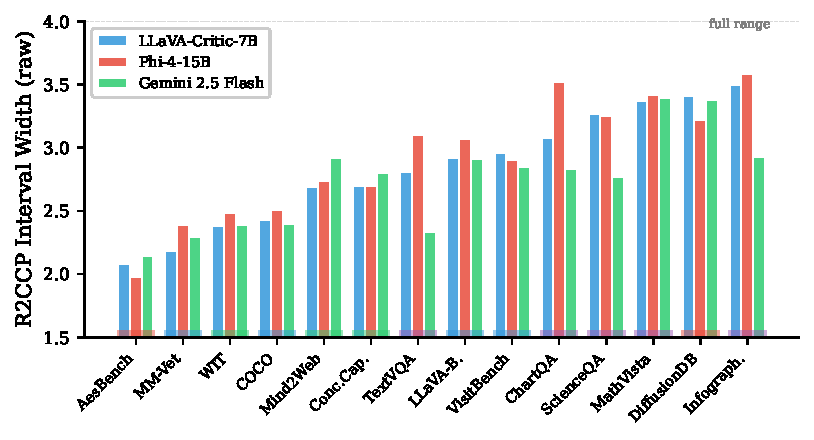
\includegraphics[width=0.8\linewidth]{figures/task_width_comparison.pdf}
\caption{R2CCP interval width across 14 task categories for all three judges. Task-dependent uncertainty is consistent: aesthetics tasks yield tight intervals while vision-heavy tasks produce wide intervals regardless of the judge. The ordering is largely preserved across judges (Spearman $\rho = 0.82$--$0.93$).\vspace{-15pt}}
\label{fig:task_width}
\end{figure}

\subsection{Ranking-scoring decoupling}
\label{sec:decoupling}

Table~\ref{tab:per_dataset} compares per-dataset correlation with interval width. ChartQA achieves the highest Pearson correlation among all 14 datasets ($\rho = 0.507$) while producing among the widest intervals (3.08). In contrast, WIT has low correlation ($\rho = 0.164$) but relatively narrow intervals (2.38). This ranking-scoring decoupling exposes a failure mode that standard evaluation metrics do not capture. A judge can correctly order responses while assigning unreliable absolute scores. For ChartQA, high correlation suggests strong performance, yet wide intervals indicate poor calibration of absolute scores. Notably, this failure mode is not well captured in standard evaluation metrics.

The effect arises because ranking depends only on monotonic consistency, while precise scoring requires accurate calibration of score magnitudes. On tasks such as chart understanding, the judge can distinguish relative quality but struggles to assign consistent absolute scores. This distinction has direct implications. For tasks where relative ordering is sufficient, correlation-based evaluation remains appropriate. For applications requiring reliable absolute scores, wide intervals indicate that point predictions are unreliable, and pairwise comparison is preferable. The decoupling is task-specific and cannot be inferred from aggregate metrics. The same pattern appears across models. For example, Gemini achieves high correlation with tight intervals on TextVQA ($\rho = 0.600$, width $= 2.33$), but low correlation with similarly wide intervals on Mind2Web ($\rho = 0.065$, width $= 2.92$), confirming that ranking quality and scoring precision are not inherently coupled.

\begin{figure}[t]
\centering
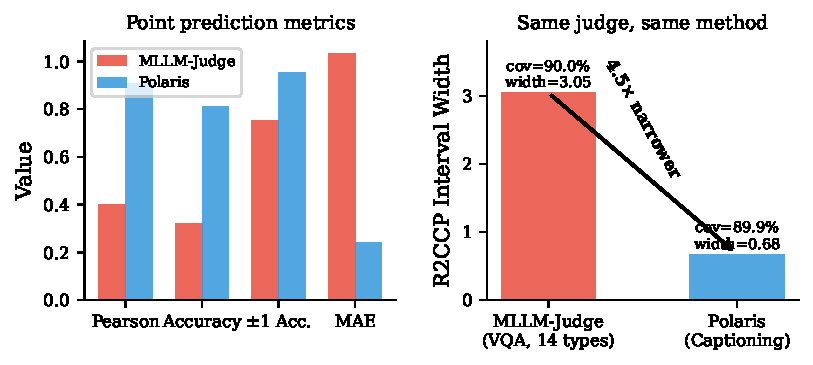
\includegraphics[width=0.7\linewidth]{figures/polaris_comparison.pdf}
\caption{MLLM-Judge vs.\ Polaris: same judge (LLaVA-Critic-7B), same CP method (R2CCP, $\alpha=0.10$), but $4.5\times$ narrower intervals when ground truth is clean (multi-annotator) and the task is well-defined (captioning). \vspace{-10pt}}
\label{fig:polaris}
\end{figure}

\begin{table}[t]
\centering
\caption{Same judge (LLaVA-Critic-7B) and method (R2CCP, $\alpha=0.10$). Multi-annotator GT and a well-defined task yield $4.5\times$ narrower intervals, while achieving 90\% coverage.}
\label{tab:polaris}
\small
\begin{tabular}{llcc}
\toprule
\textbf{Group} & \textbf{Metric} & \textbf{MLLM-Judge (14 tasks)} & \textbf{Polaris (Captioning)} \\
\midrule

Data & Samples & 5,717 & 8,726 \\
 & GT type & 1 annotator, integer & 3+ annotators, avg. \\
 & Task types & 14 visual tasks & 1 task \\

\midrule

Point & Pearson $\rho$ & .402 & \textbf{.906} \\
 & Accuracy & 32.2\% & \textbf{80.9\%} \\
 & $\pm 1$ Accuracy & 75.1\% & \textbf{95.4\%} \\
 & MAE & 1.031 & \textbf{0.243} \\
 & Bias & $+0.38$ & $\mathbf{-0.06}$ \\

\midrule

R2CCP & Coverage & .900 & .899 \\
 & \textbf{Width} & 3.05 (61\%) & \textbf{0.68 (14\%)} \\

\bottomrule\vspace{-20pt}
\end{tabular}
\end{table}

\subsection{Effect of ground truth quality: MLLM-Judge vs.\ Polaris}
\label{sec:polaris}

Table~\ref{tab:polaris} compares interval widths under identical conditions, using the same judge (LLaVA-Critic-7B) and conformal method (R2CCP with $\alpha = 0.10$). The results differ substantially: width is 3.05 on MLLM-Judge (61\% of the score range) and 0.68 on Polaris (14\%), a $4.5\times$ reduction, while both achieve the target 90\% coverage. This difference shows that interval width is primarily determined by the evaluation task and ground truth quality rather than the conformal method or model. Polaris is a single, well-defined captioning task with multi-annotator averaged labels, whereas MLLM-Judge spans diverse visual reasoning tasks with single-annotator scores. The resulting difference in signal quality is reflected directly in conformal intervals. The judge achieves substantially higher accuracy on Polaris (Pearson $= 0.906$ vs.\ $0.402$), leading to concentrated nonconformity scores and tighter intervals.

\textbf{Implications.}
When the task is well-defined and annotations are reliable, conformal prediction produces tight and actionable uncertainty estimates. Conversely, wide intervals on MLLM-Judge reflect genuine task difficulty and label noise rather than a limitation of the method. Interval width should be interpreted as an indicator of evaluation reliability.

\begin{table}[t]
\centering
\caption{Multi-judge feature fusion (R2CCP, 10 seeds). Combining judges does NOT outperform the best single judge (Gemini). Logprob quality $>$ quantity.}
\label{tab:multijudge}
\small
\begin{tabular}{lrccc}
\toprule
\textbf{Configuration} & \textbf{Feat.} & \textbf{Cov.} & \textbf{Width} & \textbf{Width} \\
& & \textbf{(raw)} & \textbf{(raw)} & \textbf{(adj.)} \\
\midrule
Gemini only & 5 & .898 & \textbf{2.85} & \textbf{3.41} \\
LLaVA + Gemini & 10 & .901 & 3.02 & 3.51 \\
LLaVA only & 5 & .900 & 3.05 & 3.60 \\
Multi-Judge (all 3) & 15 & .905 & 3.14 & 3.56 \\
LLaVA + Phi-4 & 10 & .903 & 3.18 & 3.62 \\
Phi-4 only & 5 & .891 & 3.13 & 3.70 \\
\bottomrule
\end{tabular}
\end{table}

\textbf{Multi-judge feature fusion.}
We also test whether combining logprob features from multiple judges improves conformal prediction. Contrary to expectation, fusion degrades performance: combining all three judges produces wider intervals (3.14) than using the best single judge (Gemini, 2.85). This occurs because additional features from weaker judges introduce noise without sufficient signal, making the learned nonconformity mapping less effective under limited calibration data. These results suggest that feature quality is more important than feature quantity, i.e., using a single strong judge is preferable tomultiple weaker ones.

\section{Conclusion}
\label{sec:conclusion}

We show that VLM judge reliability is governed primarily by task structure and data quality rather than the model or method. Uncertainty varies strongly across tasks and is consistent across judges. We identify a ranking-scoring decoupling where judges can rank responses correctly while assigning unreliable absolute scores, a failure mode not captured by standard metrics, and show that interval width is driven by task difficulty and annotation quality, with a $4.5\times$ reduction under clean, well-defined conditions. These findings lead to a simple operational guideline: narrow conformal intervals indicate reliable evaluation suitable for absolute scoring, while wide intervals signal ambiguity or noise where relative ranking or pairwise comparison is more appropriate. Conformal prediction thus provides a practical, uncertainty-aware framework for deploying VLM judges, with interval width serving as a direct indicator of evaluation reliability.


\pagebreak


\section*{Reproducibility statement}
All experiments use publicly available models (LLaVA-Critic-7B, Phi-4-reasoning-vision-15B) and datasets (MLLM-as-a-Judge, Polaris). Gemini 2.5 Flash is accessed via the Google Vertex AI API. We will release our complete code, including inference scripts, feature extraction pipeline, conformal prediction runners, and all result CSVs upon acceptance. Results are reported across 10 random seeds with mean $\pm$ standard deviation. All conformal prediction methods use publicly available implementations (R2CCP from the authors' wheel, MAPIE v0.8.6 for CQR variants, custom implementations following published algorithms for CHR, LVD, Boosted methods, and OrdinalAPS). Hardware: 2$\times$ RTX 6000 Ada GPUs (48GB each) for open-source model inference.

\section*{Ethics statement}
Our work analyzes the reliability of automated VLM evaluators and does not introduce new evaluation capabilities---it quantifies the uncertainty of existing ones. We note several ethical considerations: (1) Conformal prediction guarantees are marginal (averaged over the calibration/test split) rather than conditional, and should not be over-interpreted as individual-instance confidence. (2) Biased human annotations in the calibration set propagate to biased prediction intervals---conformal prediction cannot correct for systematic annotator bias. (3) The positive bias we observe (judges overscoring bad answers) may mask quality problems in deployed AI systems if interval information is ignored. We encourage practitioners to use conformal intervals as a complement to, not a replacement for, careful human evaluation in high-stakes settings.


\bibliography{references}
\bibliographystyle{colm2026_conference}

% ============================================================================
\appendix

\section{Methods and Implementation}
\label{app:methods}

\subsection{Conformal prediction methods}
\label{sec:appendix_cp_methods}

We evaluate eight conformal prediction methods spanning regression-based and classification-based approaches, following \citet{sheng2025analyzing}.

\paragraph{Regression-based methods.}
These include Naive Split Conformal Prediction, which uses absolute residuals; Conformalized Quantile Regression (CQR)~\citep{romano2019conformalized}, which learns conditional quantiles; Asymmetric CQR~\citep{sesia2019comparison}, which calibrates upper and lower bounds separately; Conformal Histogram Regression (CHR)~\citep{sesia2021conformal}, which uses histogram-based estimation; and Locally adaptive variance-based methods (LVD)~\citep{lin2021locally}. We also evaluate boosted variants of CQR and LCP~\citep{xie2025boosted}, as well as R2CCP~\citep{guha2024conformal}, which models the full conditional distribution via regression-as-classification.

\paragraph{Classification-based methods.}
We additionally consider Ordinal Adaptive Prediction Sets (OrdinalAPS)~\citep{lu2022fair}, which construct contiguous prediction sets that respect the ordinal structure of ratings.

\subsection{Feature extraction}
\label{app:feature_extraction}

For each evaluation instance, we extract the log-probabilities of the score tokens as defined in Equation~\ref{eq:features}. Because chain-of-thought outputs may contain multiple intermediate numeric tokens, identifying the final rating token is non-trivial.

We use the following heuristic:
\begin{enumerate}
\item Search for score-related keywords (e.g., ``score'', ``rating'') followed by a digit token.
\item Perform a backward scan from the end of the generated sequence to locate the final rating token.
\end{enumerate}

At the identified position, we extract the log-probabilities for all rating tokens (``1'' through ``5''), yielding a 5-dimensional feature vector per sample. For models with partial log-probability access, missing tokens are assigned a default low value.

\subsection{Evaluation prompts}
\label{app:prompts}

\subsubsection{MLLM-as-a-Judge CoT prompt}

We use a chain-of-thought prompt adapted from the MLLM-as-a-Judge dataset~\citep{chen2024mllmasajudge}. The prompt follows the ``COT figure'' setting that forces the judge to analyze the image first, then evaluate the response, then provide a final score:

\begin{quote}
\small
\textit{Please serve as an unbiased judge in assessing the quality of the response from an AI assistant regarding the user's instruction and the provided image.}

\textit{Evaluation Steps: Please examine the provided image attentively. Begin by conducting a comprehensive analysis of the figure provided. Then, utilize the insights from your analysis to critically evaluate the response. Finally, based on your figure analysis and response evaluation, form a well-reasoned judgement.}

\textit{Scoring Rubric:}
\textit{Poor (1): The response significantly deviates from the user's instruction and fails to address the query effectively. It shows a lack of relevance, accuracy, and comprehensiveness. Creativity and granularity are absent or poorly executed.}
\textit{Fair (2): The response addresses the user's instruction partially, with evident shortcomings in relevance, accuracy, or comprehensiveness. It lacks depth in creativity and granularity.}
\textit{Average (3): The response adequately addresses the user's instruction, showing a fair level of relevance, accuracy, and comprehensiveness. It reflects a basic level of creativity and granularity but may lack sophistication.}
\textit{Good (4): The response is well-aligned with the user's instruction, demonstrating a high degree of relevance, accuracy, and comprehensiveness. It shows creativity and nuanced understanding.}
\textit{Excellent (5): The response perfectly adheres to the user's instruction, excelling in relevance, accuracy, comprehensiveness, creativity, and granularity.}

\textit{Notice: In your evaluation, weigh factors such as relevance, accuracy, comprehensiveness, creativity, and the granularity of the response. Do not allow the length of the response to influence your evaluation. Be as objective as possible.}

\textit{Here is the input:}
\textit{[The Start of User Instruction] \{question\} [The End of User Instruction]}
\textit{[The Start of Assistant's Answer] \{actor\_answer\} [The End of Assistant's Answer]}

\textit{First, provide your analysis of the image and the response. Then, at the very end of your response, provide your final score in exactly this format on its own line: ``Score: X'' where X is a single number from 1 to 5.}
\end{quote}

\subsubsection{Polaris captioning prompt}

For the Polaris captioning dataset, we adapt the prompt structure for caption evaluation:

\begin{quote}
\small
\textit{Please serve as an unbiased judge in assessing the quality of an image caption generated by an AI model.}

\textit{Evaluation Steps: Please examine the provided image attentively. Then evaluate how well the generated caption describes the image content.}

\textit{Scoring Rubric:}
\textit{Poor (1): The caption is completely inaccurate, irrelevant, or fails to describe the image content. Major factual errors or hallucinations are present.}
\textit{Fair (2): The caption partially describes the image but has significant inaccuracies, missing key elements, or includes incorrect details.}
\textit{Average (3): The caption adequately describes the main content of the image with fair accuracy, but may miss some details or include minor inaccuracies.}
\textit{Good (4): The caption accurately describes the image content with good detail and relevance, with only minor omissions.}
\textit{Excellent (5): The caption perfectly describes the image content with high accuracy, comprehensive detail, and excellent relevance to what is shown.}

\textit{Provide your analysis of how well the caption matches the image, then provide your final score in exactly this format on its own line: ``Score: X'' where X is a single number from 1 to 5.}
\end{quote}

\section{Core Results}

\subsection{Cross-Judge Comparison}
\label{app:all_methods}

Table~\ref{tab:all_methods_all_judges} compares the top conformal methods across all three judges. R2CCP and CHR consistently achieve the best coverage-width tradeoff. Gemini produces the narrowest intervals across methods, indicating better-calibrated score distributions.

\begin{table}[t]
\centering
\caption{Top CP methods across judges (raw coverage and width, 10 seeds).}
\label{tab:all_methods_all_judges}
\small
\begin{tabular}{lcccccc}
\toprule
& \multicolumn{2}{c}{\textbf{LLaVA-Critic}} & \multicolumn{2}{c}{\textbf{Phi-4}} & \multicolumn{2}{c}{\textbf{Gemini}} \\
\cmidrule(lr){2-3} \cmidrule(lr){4-5} \cmidrule(lr){6-7}
\textbf{Method} & Cov. & Width & Cov. & Width & Cov. & Width \\
\midrule
R2CCP & .900 & 3.05 & .891 & 3.13 & .898 & \textbf{2.85} \\
CHR & .880 & 2.97 & .896 & 3.16 & .880 & \textbf{2.80} \\
B.\ LCP & .863 & 3.02 & .875 & 3.24 & .863 & \textbf{2.88} \\
Naive CP & .895 & 3.23 & .897 & 3.30 & .893 & \textbf{3.08} \\
CQR & .996 & 3.95 & .997 & 3.98 & .996 & 3.95 \\
\bottomrule
\end{tabular}
\end{table}

\subsection{Per-Dataset Results}
\label{app:per_dataset_core}

\textbf{Width comparison across judges.}
Table~\ref{tab:all_judges_per_dataset} shows per-dataset interval widths. Gemini yields the narrowest intervals on 10 of 14 datasets, with the largest gains on vision-heavy tasks, indicating better alignment between ranking and scoring.

\begin{table}[t]
\centering
\caption{Per-dataset R2CCP raw width for all three judges. Bold indicates the narrowest width for each dataset.}
\label{tab:all_judges_per_dataset}
\small
\begin{tabular}{lcccc}
\toprule
\textbf{Dataset} & \textbf{LLaVA} & \textbf{Phi-4} & \textbf{Gemini} & \textbf{Cat.} \\
\midrule
AesBench & 2.08 & \textbf{1.98} & 2.14 & Aesth. \\
MM-Vet & \textbf{2.18} & 2.39 & 2.29 & Gen. \\
WIT & \textbf{2.38} & 2.48 & 2.39 & Know. \\
COCO & 2.43 & 2.51 & \textbf{2.40} & Gen. \\
Mind2Web & \textbf{2.69} & 2.74 & 2.92 & Know. \\
Conc.\ Cap. & 2.70 & \textbf{2.70} & 2.80 & Know. \\
TextVQA & 2.81 & 3.10 & \textbf{2.33} & Vision \\
LLaVA-B. & 2.92 & 3.07 & \textbf{2.91} & Gen. \\
VisitBench & 2.96 & 2.90 & \textbf{2.85} & Gen. \\
ChartQA & 3.08 & 3.52 & \textbf{2.83} & Vision \\
ScienceQA & 3.27 & 3.25 & \textbf{2.77} & Vision \\
MathVista & 3.37 & 3.42 & \textbf{3.39} & Vision \\
DiffusionDB & 3.41 & \textbf{3.22} & 3.38 & Aesth. \\
Infograph. & 3.50 & 3.58 & \textbf{2.93} & Vision \\
\midrule
\textbf{Overall} & 3.05 & 3.13 & \textbf{2.85} & --- \\
\bottomrule
\end{tabular}
\end{table}

\textbf{Relaxed accuracy and MAE.}
Table~\ref{tab:relaxed_accuracy} reports relaxed accuracy ($\pm 1$) and MAE. While higher accuracy generally correlates with narrower intervals, several datasets violate this trend, confirming that ranking quality and scoring precision are not tightly coupled.

\begin{table}[t]
\centering
\caption{Per-dataset relaxed accuracy and MAE for LLaVA-Critic-7B.}
\label{tab:relaxed_accuracy}
\small
\begin{tabular}{lccccc}
\toprule
\textbf{Dataset} & \textbf{N} & \textbf{Exact} & $\pm 1$ & \textbf{MAE} & \textbf{Bias} \\
\midrule
AesBench & 392 & 41.3\% & 88.3\% & 0.732 & $+0.49$ \\
COCO & 397 & 34.5\% & 84.9\% & 0.854 & $+0.04$ \\
Conc.\ Cap. & 398 & 35.4\% & 81.7\% & 0.872 & $+0.60$ \\
LLaVA-B. & 396 & 31.8\% & 81.1\% & 0.922 & $+0.55$ \\
MM-Vet & 258 & 37.2\% & 80.2\% & 0.926 & $-0.01$ \\
TextVQA & 399 & 36.3\% & 79.2\% & 0.942 & $+0.30$ \\
WIT & 399 & 33.8\% & 78.7\% & 0.912 & $+0.51$ \\
VisitBench & 397 & 31.7\% & 75.1\% & 1.018 & $+0.44$ \\
Mind2Web & 398 & 29.6\% & 74.4\% & 1.008 & $+0.19$ \\
ChartQA & 400 & 30.2\% & 73.2\% & 1.085 & $+0.31$ \\
ScienceQA & 396 & 26.5\% & 69.7\% & 1.200 & $+0.30$ \\
Infograph. & 398 & 25.1\% & 69.3\% & 1.191 & $+0.18$ \\
MathVista & 789 & 32.3\% & 65.1\% & 1.235 & $+0.33$ \\
DiffusionDB & 299 & 23.7\% & 57.2\% & 1.385 & $+1.23$ \\
\bottomrule
\end{tabular}
\end{table}

\textbf{Confusion matrices.}
Table~\ref{tab:confusion} reveals distinct error patterns across judges. LLaVA exhibits broad dispersion, Phi-4 gravitates toward score 4, and Gemini polarizes between scores 1 and 5.

\begin{table}[t]
\centering
\caption{Row-normalized confusion matrices (\%, GT rows, Pred columns).}
\label{tab:confusion}
\small
\begin{tabular}{l|ccccc|c}
\toprule
& \textbf{P=1} & \textbf{P=2} & \textbf{P=3} & \textbf{P=4} & \textbf{P=5} & $\pm 1$ \\
\midrule
\multicolumn{7}{l}{\emph{LLaVA-Critic-7B}} \\
GT=1 & 32.6 & 12.9 & 17.0 & 23.4 & 14.0 & 45.6 \\
GT=2 & 17.0 & 11.7 & 21.9 & 32.2 & 17.1 & 50.6 \\
GT=3 & 5.2 & 7.0 & 18.6 & 42.0 & 27.2 & 67.6 \\
GT=4 & 3.3 & 3.6 & 13.4 & 38.9 & 40.8 & 93.1 \\
GT=5 & 1.9 & 2.2 & 10.7 & 38.4 & 46.7 & 85.2 \\
\bottomrule
\end{tabular}
\end{table}

\subsection{Polaris Results}
\label{app:polaris_core}

\textbf{Confusion matrix.}
Table~\ref{tab:polaris_confusion} shows near-perfect identification of low-quality captions (GT = 1), with most confusion between adjacent categories.

\begin{table}[t]
\centering
\caption{Confusion matrix for Polaris (\%).}
\label{tab:polaris_confusion}
\small
\begin{tabular}{l|ccccc|c}
\toprule
& \textbf{P=1} & \textbf{P=2} & \textbf{P=3} & \textbf{P=4} & \textbf{P=5} & $\pm 1$ \\
\midrule
GT=1 & 99.6 & 0.1 & 0.2 & 0.1 & 0.0 & 99.7 \\
GT=2 & 74.2 & 12.9 & 5.7 & 4.8 & 2.4 & 92.7 \\
GT=3 & 18.6 & 13.4 & 32.1 & 30.8 & 5.2 & 76.2 \\
GT=4 & 1.6 & 4.0 & 14.6 & 64.2 & 15.6 & 94.4 \\
GT=5 & 0.8 & 2.0 & 5.6 & 63.9 & 27.8 & 91.7 \\
\bottomrule
\end{tabular}
\end{table}

\textbf{Error-bin CP coverage.}
Table~\ref{tab:polaris_error_bins} shows that tight intervals reduce raw coverage for $\pm 1$ errors, but boundary adjustment restores coverage to near-perfect levels.

\begin{table}[t]
\centering
\caption{CP coverage by error magnitude on Polaris.}
\label{tab:polaris_error_bins}
\small
\begin{tabular}{lccc}
\toprule
\textbf{Error} & \textbf{\% samples} & \textbf{Cov. (raw)} & \textbf{Cov. (adj.)} \\
\midrule
Exact (0) & 80.9\% & 98.2\% & 99.6\% \\
$\pm 1$ & 14.6\% & 58.1\% & 99.4\% \\
$\pm 2$ & 4.1\% & 50.0\% & 80.7\% \\
$\pm 3$ & 0.5\% & 0.6\% & 52.4\% \\
\bottomrule
\end{tabular}
\end{table}

\section{Diagnostics and Analysis}

\textbf{Error Analysis.}
Figure~\ref{fig:error_bins} and Table~\ref{tab:error_bins} show conformal prediction behavior conditioned on judge error magnitude. CP is most effective when the judge is wrong: boundary-adjusted coverage exceeds 99\% for $\pm 1$ and $\pm 2$ errors, which constitute the majority of mistakes. Overall, CP recovers 97.8\% of all judge errors. 

\begin{figure}[t]
\centering
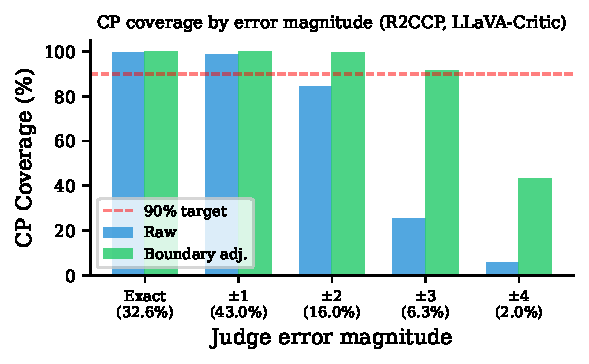
\includegraphics[width=0.6\linewidth]{figures/error_bin_coverage.pdf}
\caption{CP coverage by error magnitude. Boundary adjustment is critical: for $\pm 2$ errors, raw coverage is 84\% but adjusted coverage reaches 99\%.}
\label{fig:error_bins}
\end{figure}

\begin{table}[t]
\centering
\caption{CP coverage by error magnitude (R2CCP, LLaVA-Critic-7B).}
\label{tab:error_bins}
\small
\begin{tabular}{lccccc}
\toprule
\textbf{Error} & \textbf{\% samp.} & \textbf{Cov. (raw)} & \textbf{Cov. (adj.)} & \textbf{Width (raw)} & \textbf{Width (adj.)} \\
\midrule
0 (exact) & 32.6\% & 99.8\% & 100\% & 2.98 & 3.55 \\
$\pm 1$ & 43.0\% & 98.7\% & 99.9\% & 3.08 & 3.63 \\
$\pm 2$ & 16.0\% & 84.3\% & 99.4\% & 3.12 & 3.65 \\
$\pm 3$ & 6.3\% & 25.4\% & 91.5\% & 3.05 & 3.61 \\
$\pm 4$ & 2.0\% & 5.7\% & 43.3\% & 2.89 & 3.42 \\
\midrule
\multicolumn{6}{l}{\emph{Overall: 97.8\% recovery}} \\
\bottomrule
\end{tabular}
\end{table}

\textbf{Bias Analysis.}
Table~\ref{tab:bias} shows mean signed error conditioned on ground truth score. All judges overscore low-quality responses and underscore high-quality responses, producing compression toward mid-range scores. This bias explains the asymmetry in error distributions.

\begin{table}[t]
\centering
\caption{Mean signed error by ground truth score level.}
\label{tab:bias}
\small
\begin{tabular}{lccc}
\toprule
\textbf{GT Score} & \textbf{LLaVA} & \textbf{Phi-4} & \textbf{Gemini} \\
\midrule
1 & $+1.73$ & $+1.98$ & $\mathbf{+0.89}$ \\
2 & $+1.21$ & $+1.13$ & $\mathbf{+0.43}$ \\
3 & $+0.79$ & $+0.34$ & $\mathbf{+0.23}$ \\
4 & $+0.10$ & $-0.35$ & $\mathbf{-0.15}$ \\
5 & $-0.74$ & $-1.04$ & $\mathbf{-0.87}$ \\
\midrule
\textbf{Overall} & $+0.38$ & $+0.08$ & $\mathbf{-0.05}$ \\
\bottomrule
\end{tabular}
\end{table}

\textbf{Ranking-Scoring Decoupling.}
Table~\ref{tab:rsg} and Figure~\ref{fig:decoupling} show that ranking quality and scoring precision are not coupled. High correlation does not imply narrow intervals. Coverage is weakest for GT = 1 due to systematic overscoring, while other levels achieve near-perfect adjusted coverage.

\begin{table}[t]
\centering
\caption{Ranking-Scoring Gap (RSG). Positive values indicate strong ranking but weak scoring precision.}
\label{tab:rsg}
\small
\begin{tabular}{lcccccc}
\toprule
& \multicolumn{2}{c}{\textbf{LLaVA}} & \multicolumn{2}{c}{\textbf{Phi-4}} & \multicolumn{2}{c}{\textbf{Gemini}} \\
\cmidrule(lr){2-3} \cmidrule(lr){4-5} \cmidrule(lr){6-7}
\textbf{Dataset} & $\rho$ & RSG & $\rho$ & RSG & $\rho$ & RSG \\
\midrule
Infograph. & .411 & \textbf{+.287} & .162 & +.058 & .547 & \textbf{+.281} \\
ChartQA & .507 & \textbf{+.276} & .261 & +.141 & .494 & \textbf{+.201} \\
MathVista & .376 & \textbf{+.219} & .339 & +.194 & .414 & \textbf{+.262} \\
VisitBench & .352 & +.091 & .339 & +.064 & .524 & +.235 \\
ScienceQA & .258 & +.075 & .304 & +.115 & .530 & +.223 \\
TextVQA & .389 & +.092 & .213 & $-$.012 & .600 & +.183 \\
\midrule
WIT & .164 & $-$.242 & .400 & +.021 & .294 & $-$.109 \\
MM-Vet & .260 & $-$.195 & .296 & $-$.108 & .233 & $-$.194 \\
AesBench & .402 & $-$.077 & .353 & $-$.153 & .256 & $-$.208 \\
\bottomrule
\end{tabular}
\end{table}

\begin{figure}[t]
\centering
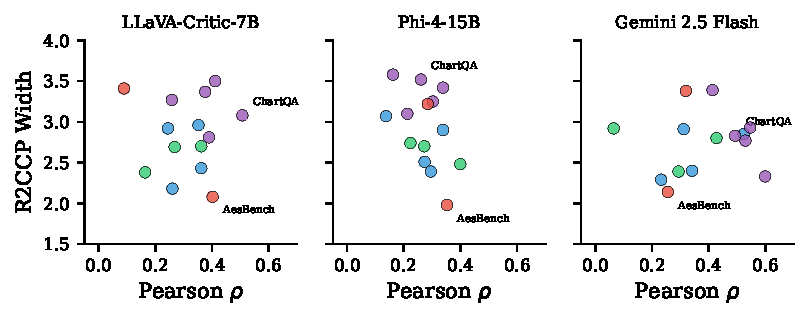
\includegraphics[width=\linewidth]{figures/ranking_scoring_decoupling.pdf}
\caption{Ranking-scoring decoupling across datasets. High correlation does not imply reliable absolute scores.}
\label{fig:decoupling}
\end{figure}

\textbf{Conditional Coverage.}
Table~\ref{tab:conditional} shows coverage conditioned on ground truth score. As shown in Table~\ref{tab:conditional}, coverage is lowest for GT = 1, while other levels achieve near-perfect adjusted coverage.

\begin{table}[t]
\centering
\caption{Conditional coverage by ground truth score.}
\label{tab:conditional}
\small
\begin{tabular}{lcccccc}
\toprule
\textbf{GT} & \textbf{N} & \textbf{Cov. (raw)} & \textbf{Cov. (adj.)} & \textbf{Width (raw)} & \textbf{Width (adj.)} & \textbf{Bias} \\
\midrule
1 & 334 & 53.0\% & 88.9\% & 3.14 & 3.75 & +1.67 \\
2 & 360 & 86.9\% & 100\% & 3.18 & 3.79 & +1.13 \\
3 & 637 & 99.7\% & 100\% & 3.09 & 3.75 & +0.77 \\
4 & 880 & 98.2\% & 100\% & 2.99 & 3.65 & +0.11 \\
5 & 648 & 92.4\% & 99.2\% & 2.92 & 3.58 & -0.80 \\
\bottomrule
\end{tabular}
\end{table}

\section{Ablations}

\textbf{Mondrian Conformal Prediction.}
Table~\ref{tab:mondrian} shows results for Mondrian conformal prediction, which computes group-specific quantiles based on task difficulty. Compared to standard R2CCP, Mondrian CP produces narrower intervals for easier tasks and improved coverage for harder ones. Easy tasks receive 16.6\% narrower intervals, while hard tasks achieve higher coverage, reducing unnecessary conservativeness.

\textbf{Naive Split CP vs.\ R2CCP.}
Table~\ref{tab:naive_vs_r2ccp} shows that R2CCP consistently outperforms the Naive Split CP baseline across all datasets, producing uniformly narrower intervals.

\begin{table}[t]
\centering
\caption{Naive Split CP vs.\ R2CCP per dataset (raw width, LLaVA-Critic-7B).}
\label{tab:naive_vs_r2ccp}
\small
\begin{tabular}{lccc}
\toprule
\textbf{Dataset} & \textbf{Naive} & \textbf{R2CCP} & $\Delta$ \\
\midrule
AesBench & 2.53 & \textbf{2.08} & $-0.45$ \\
MM-Vet & 3.39 & \textbf{2.18} & $-1.21$ \\
WIT & 2.92 & \textbf{2.38} & $-0.54$ \\
COCO & 2.86 & \textbf{2.43} & $-0.43$ \\
Mind2Web & 3.13 & \textbf{2.69} & $-0.44$ \\
Conc.\ Cap. & 3.11 & \textbf{2.70} & $-0.41$ \\
TextVQA & 3.19 & \textbf{2.81} & $-0.38$ \\
LLaVA-B. & 3.28 & \textbf{2.92} & $-0.36$ \\
VisitBench & 3.37 & \textbf{2.96} & $-0.41$ \\
ChartQA & 3.49 & \textbf{3.08} & $-0.41$ \\
ScienceQA & 3.71 & \textbf{3.27} & $-0.44$ \\
MathVista & 3.64 & \textbf{3.37} & $-0.27$ \\
DiffusionDB & 3.56 & \textbf{3.41} & $-0.15$ \\
Infograph. & 3.67 & \textbf{3.50} & $-0.17$ \\
\midrule
\textbf{Average} & 3.27 & \textbf{2.84} & $-0.42$ \\
\bottomrule
\end{tabular}
\end{table}

\textbf{Effect of Chain-of-Thought Prompting.}
Table~\ref{tab:cot_effect} shows that CoT improves correlation metrics and significantly reduces overconfidence, providing better signal for conformal prediction.

\begin{table}[t]
\centering
\caption{Effect of CoT prompting on LLaVA-Critic-7B.}
\label{tab:cot_effect}
\small
\begin{tabular}{lcc}
\toprule
\textbf{Metric} & \textbf{Generic} & \textbf{CoT} \\
\midrule
Pearson $\rho$ & .380 & \textbf{.402} ($+5.8\%$) \\
Spearman $\rho_s$ & .314 & \textbf{.356} ($+13.4\%$) \\
Kendall $\tau$ & .270 & \textbf{.300} ($+11.1\%$) \\
Exact accuracy & \textbf{33.9\%} & 32.2\% \\
MAE & 1.058 & \textbf{1.031} \\
\midrule
Overconf.\ ($>$0.99) & 51.4\% & \textbf{25.6\%} ($-50\%$) \\
Overconf.\ ($>$0.999) & 33.2\% & \textbf{6.6\%} ($-80\%$) \\
\bottomrule
\end{tabular}
\end{table}

% \textbf{Multi-Judge Fusion.} Combining predictions from multiple judges can improve robustness by averaging out individual biases and uncertainties. Preliminary analysis suggests that fusion reduces variance in interval estimates and improves coverage stability, though detailed evaluation is left for future work.

\section{Additional Observations}

\textbf{Interval Informativeness.}
On MLLM-Judge, 0.5\% of intervals are decisive, 30.7\% are moderately informative, and 68.8\% are uninformative. In contrast, Polaris produces mostly decisive intervals due to stronger signal quality.

\textbf{Midpoint Analysis.}
Table~\ref{tab:midpoint} shows that midpoint-based estimates do not consistently outperform raw scores due to wide intervals.

\begin{table}[t]
\centering
\caption{Midpoint vs raw score.}
\label{tab:midpoint}
\small
\begin{tabular}{lccc}
\toprule
\textbf{Metric} & \textbf{Raw} & \textbf{Midpoint} & \textbf{Adj.\ Mid} \\
\midrule
Pearson & .412 & .396 & .277 \\
Spearman & .367 & .359 & .272 \\
MAE & 1.022 & .992 & 1.056 \\
Accuracy & 32.6\% & --- & 28.1\% \\
\bottomrule
\end{tabular}
\end{table}

\end{document}
